\documentclass{article}
\usepackage{titlesec}
\usepackage{graphicx}
\usepackage{fancyhdr}
\usepackage{multirow}
\usepackage{colortbl}
\usepackage{hhline}
\usepackage{lipsum}
\usepackage[sorting=none]{biblatex}
 \usepackage{float}
\usepackage[margin=1in]{geometry}
\usepackage{listings}
\usepackage[hidelinks]{hyperref}
\usepackage{xcolor}
\usepackage{subfigure}


 \usepackage{color}
  \usepackage{rotating}
\usepackage{tabularray}

\definecolor{ScreaminGreen}{rgb}{0.4,0.941,0.607}
\definecolor{Canary}{rgb}{0.862,1,0.36}
\definecolor{CottonCandy}{rgb}{1,0.741,0.905}
\definecolor{BilobaFlower}{rgb}{0.654,0.662,0.925}
\definecolor{Cherub}{rgb}{0.956,0.803,0.925}

\usepackage{xepersian}


%\addbibresource{bibliography.bib}
\settextfont{Times New Roman}
\settextfont[Scale=1.2]{HM_FZar.ttf}
\setlatintextfont[Scale=1]{Times New Roman}

\renewcommand{\baselinestretch}{1.5}

\pagestyle{fancy}
\fancyhf{}
%\fancyhead{}
%\fancyhead[]{\rightmark}
\renewcommand{\sectionmark}[1]{\markright{#1}}
\fancyhead[L]{\nouppercase{\rightmark}}
\fancyhead[R]{پاسخ تمارین سری 1 و 2 سیستم های چندرسانه‌ای پیشرفته}



\cfoot{\thepage}
\renewcommand{\headrulewidth}{1pt}
\renewcommand{\footrulewidth}{1pt}

\begin{document}
	%\thispagestyle{plain}

\begin{titlepage}
	
	\begin{center}
		
        	
\includegraphics[width=0.2\textwidth]{iut.png}

		\large
		دانشکده مهندسی برق و کامپیوتر
		
		\vfill
		\Large
		
		\textbf{سیستم‌های چندرسانه‌ای پیشرفته}
		\\
	
		\vfill
		
		\large
\textbf{پاسخ تمرین سری 1 و 2}
		\vfill

		
		نام و نام خانوادگی دانشجو: قوام سلیمانی


\vfill
پاییز 1402
	\end{center}
\end{titlepage}

	
	\tableofcontents
	\newpage
	
	\section{پاسخ سوال اول}
مراجع \cite{1} \cite{2} \cite{3}
	\subsection{کاربرد هر \lr{Format}}
همۀ این فایل‌ها به طور گسترده برای ذخیره و نمایش تصاویر در برنامه‌های گوناگون براساس بیت مپ های ساده بلافاصله پس از \lr{Header} مورد استفاده قرار می گیرند که به علت این ساختار ساده، قابل حمل نامیده می شوند و به راحتی در دستگاه های مختلف مورد استفاده قرار می گیرند. در ادامه به صورت جداگانه بررسی می شوند.

\begin{enumerate}
\item \lr{PPM}\\
فایل‌های \lr{PPM} تصاویر تمام رنگی یا \lr{RGB} (قرمز، سبز، آبی) را نمایش می‌دهند. آنها اطلاعات رنگ هر پیکسل را به صورت جداگانه ذخیره می کنند. فرمت \lr{PPM} اغلب در زمینه هایی مانند ویرایش تصویر و گرافیک کامپیوتری استفاده می شود. این فرمت از طیف گسترده ای از رنگ ها پشتیبانی می کند و فقط به تصاویر سیاه و سفید یا باینری محدود نمی شود.


\item \lr{PGM}\\
فرمت \lr{PGM} برای تصاویر خاکستری استفاده می شود. هر پیکسل را با یک مقدار عددی جهت نمایش رنگ خاکستری، (از سیاه تا سفید) نشان داده می شود. فایل‌های \lr{PGM} معمولاً در الگوریتم‌های پردازش تصویر و \lr{OCR} استفاده می‌شوند که در آن اطلاعات رنگ مورد نیاز ما نخواهد بود یا تمرکز بر شدت روشنایی است.

\item \lr{PBM}\\
فرمت \lr{PBM} برای تصاویر سیاه و سفید یا باینری طراحی شده است. هر پیکسل، سیاه یا سفید را نشان می دهد. فایل های \lr{PBM} اغلب در برنامه هایی استفاده می شوند که به نمایش های تک رنگ ساده نیاز دارند، مانند دستگاه های فکس و چاپگرها، سیستم های \lr{OCR}

\end{enumerate}

	\subsection{ساختار \lr{Header} و نحوۀ ذخیره‌سازی}

	\begin{enumerate}
		\item \lr{PPM}\\
	هدر یک فایل \lr{PPM} با مقدار "\lr{P6}" برای تصاویر باینری و "\lr{P3}" برای تصاویر اسکی درنظر گرفته می‌شود و سپس عرض و ارتفاع تصویر برحسب پیکسل و حداکثر مقدار رنگ (از 0 تا 255 برای هر کانال) شروع می شود. پس از هدر، داده های تصویر به صورت سه گانه  \lr{RGB} ذخیره می شوند (16777216 رنگ).
	مثال : 
	\begin{latin}
\begin{verbatim}
P3
# Comment (Pixel storage: r1 g1 b1 r2 g2 b2 r3 g3 b3 ...)
4 4
15
0 0 0 0 0 0 0 0 0 0 15 0 15
0 0 0 0 15 7 0 0 0 0 0 0 0
0 0 0 0 0 0 0 15 7 0 0 0
15 0 15 0 0 0 0 0 0 0 0 0 0
\end{verbatim}
			\end{latin}
		
		\item \lr{PGM}
		
		هدر یک فایل \lr{PGM} با مقدار "\lr{P5}" برای تصاویر باینری و "\lr{P2}" برای تصاویر اسکی درنظر گرفته می‌شود و سپس عرض و ارتفاع تصویر برحسب پیکسل و حداکثر مقدار رنگ خاکستری (از 0 تا 255) شروع می شود. پس از هدر، داده های تصویر به صورت مقادیر پیکسل های خاکستری ذخیره می شوند.
		مثال : 
		\begin{latin}
			\begin{verbatim}
			P2
			# Comment
			24 7
			15
			0 0 0 0 0 0 0 0 0 0 0 0 0 0 0 0 0 0 0 0 0 0 0 0
			0 3 3 3 3 0 0 7 7 7 7 0 0 11 11 11 11 0 0 15 15 15 15 0
			0 3 0 0 0 0 0 7 0 0 0 0 0 11 0 0 0 0 0 15 0 0 15 0
			0 3 3 3 0 0 0 7 7 7 0 0 0 11 11 11 0 0 15 15 15 15 0
			0 3 0 0 0 0 0 7 0 0 0 0 0 11 0 0 0 0 0 15 0 0 0 0
			0 3 0 0 0 0 0 7 7 7 7 0 0 11 11 11 11 0 0 15 0 0 0 0
			0 0 
			\end{verbatim}
		\end{latin}

		
		\item \lr{PBM}
		
		هدر یک فایل \lr{PBM} با مقدار "\lr{P1}" برای تصاویر سیاه و سفید باینری درنظر گرفته می‌شود که تنها دو رنگ سیاه و سفید را نشان می دهد و سپس عرض و ارتفاع تصویر برحسب پیکسل درج می شود. پس از هدر، داده های تصویر به صورت پیکسل های سیاه و سفید ذخیره و نمایش داده می شوند.
		مثال : 
		\begin{latin}
			\begin{verbatim}
		P1
		# Comment
		6 10
		0 0 0 0 1 0
		0 0 0 0 1 0
		0 0 0 0 1 0
		0 0 0 0 1 0
		0 0 0 0 1 0
		0 0 0 0 1 0
		1 0 0 0 1 0
		0 1 1 1 0 0
		0 0 0 0 0 0
		0 0 0 0 0 0
			\end{verbatim}
		\end{latin}


	\end{enumerate}
	

	\subsection{نحوۀ ذخیره‌سازی داده‌ها}
	
	\section{خواندن \lr{PPM} در \lr{Matlab} بدون \lr{imread}}

\lr{\lstinputlisting[language=Matlab, showstringspaces=false, basicstyle=\ttfamily, backgroundcolor=\color{gray!20!white}, breaklines=true]{q2.m}}

پس از بازگشایی فایل \lr{PPM} و چک کردن نوع، باید \lr{Header} های فایل را بخوانیم. بعد از آن با توجه به اینکه به تعداد (عرض * ارتفاع * کانال های رنگی ) پیکسل داریم، داده ها را خوانده و ضمنا برای آن عددها از نوع بدون علامت 8 بیتی  صحیح استفاده می کنیم که برای این کار از \lr{fread} بهره بردیم. سپس مقادیر خوانده شده برای نمایش در حالت استاندارد، بعد اولشان نشان دهنده ی کانال های رنگی بوده سپس ارتفاع و بعد عرض. پس آن را \lr{ReShape}  کردیم. رنگ ها به هم ریخت، پس کانال های سبز و آبی را نیز جا به جا کردیم. \cite{4}

نتیجه: 
\begin{figure}[H]
	\centering
	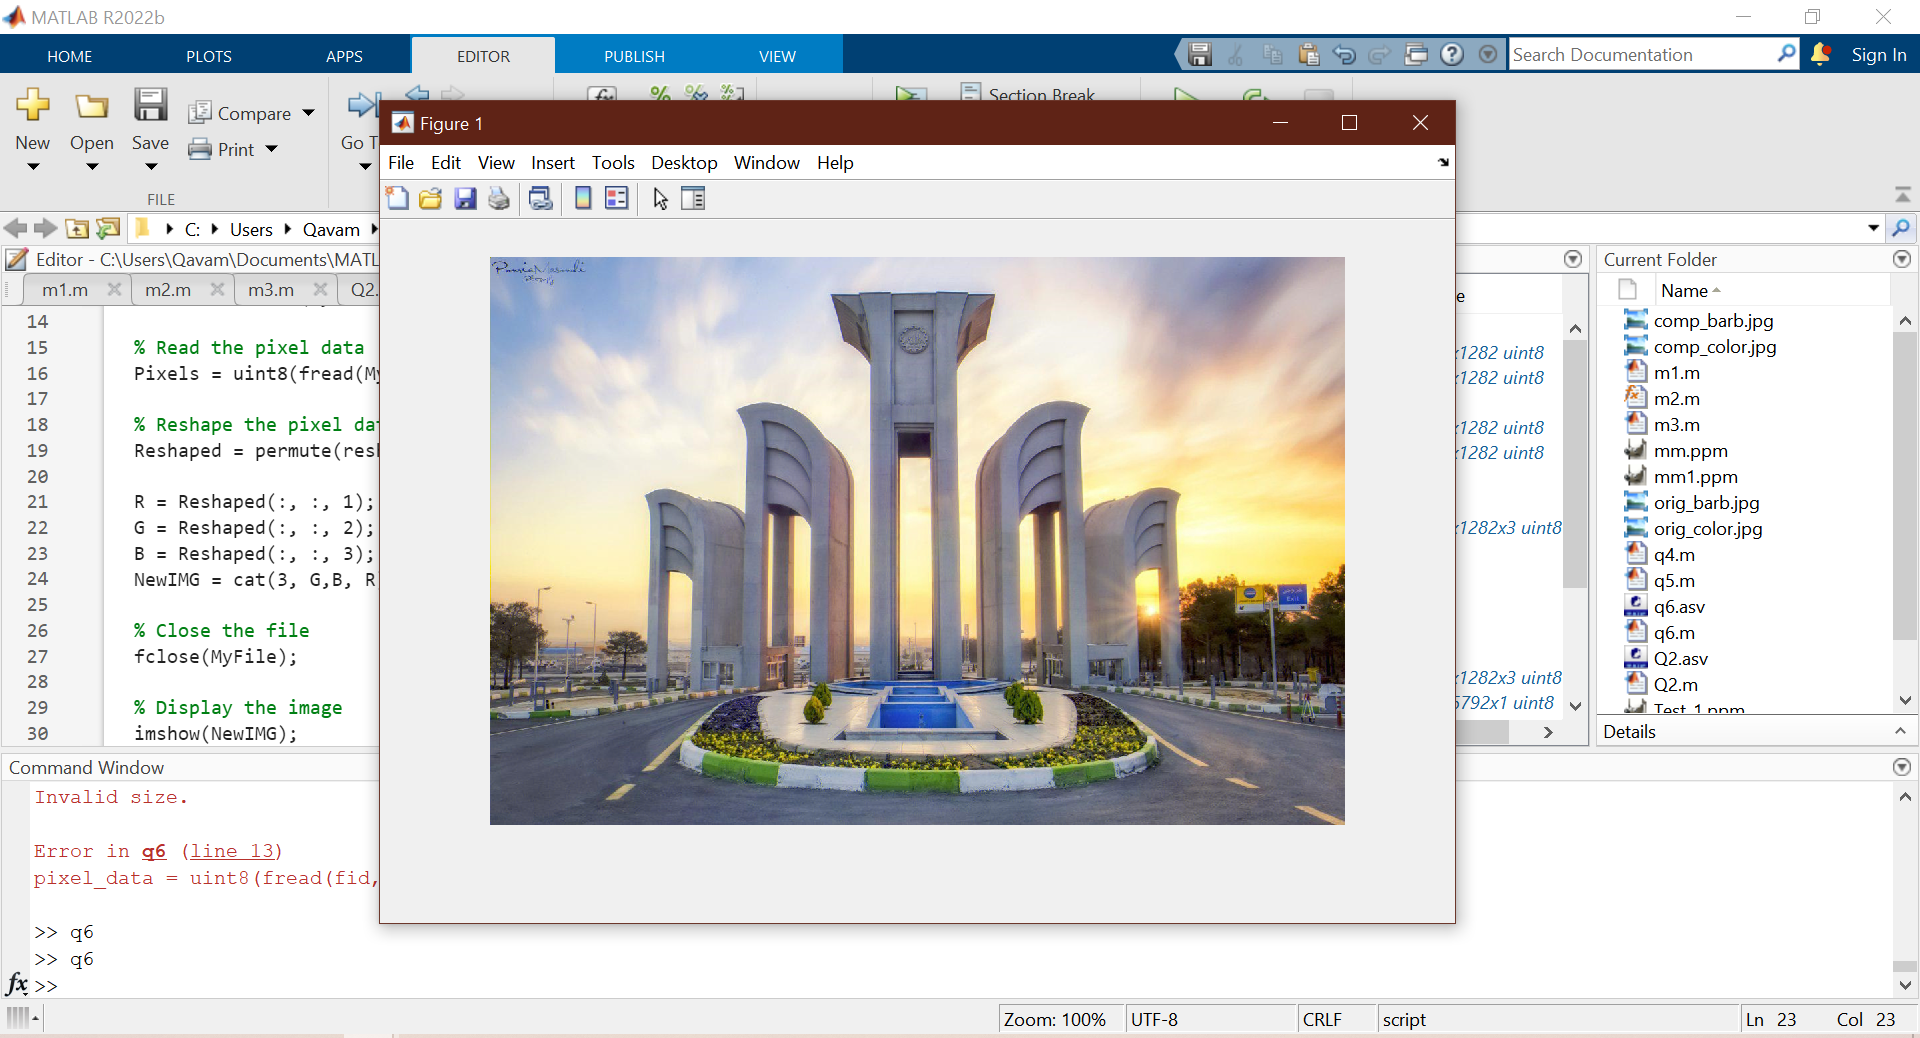
\includegraphics[width=0.9\textwidth]{1.png}
	\caption{1}
\end{figure}

\begin{figure}[H]
	\centering
	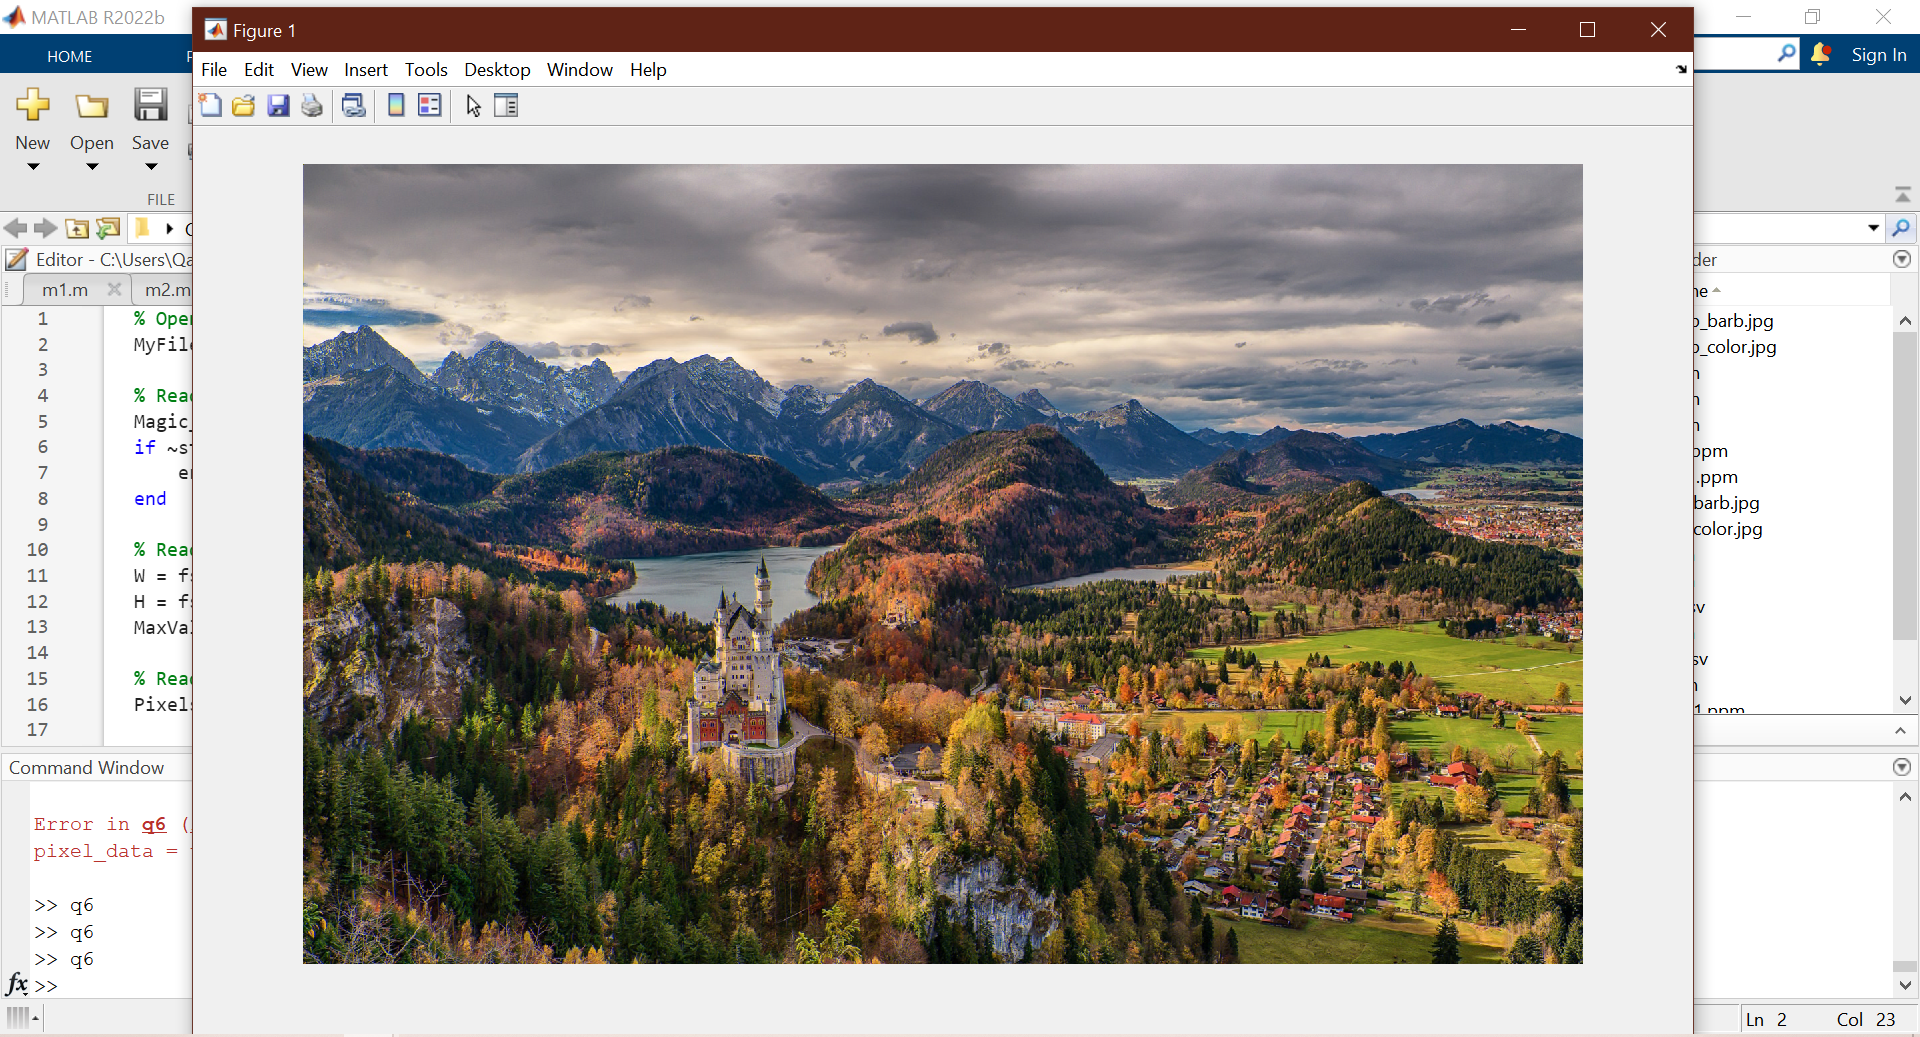
\includegraphics[width=0.9\textwidth]{2.png}
	\caption{1}
\end{figure}

\begin{figure}[H]
	\centering
	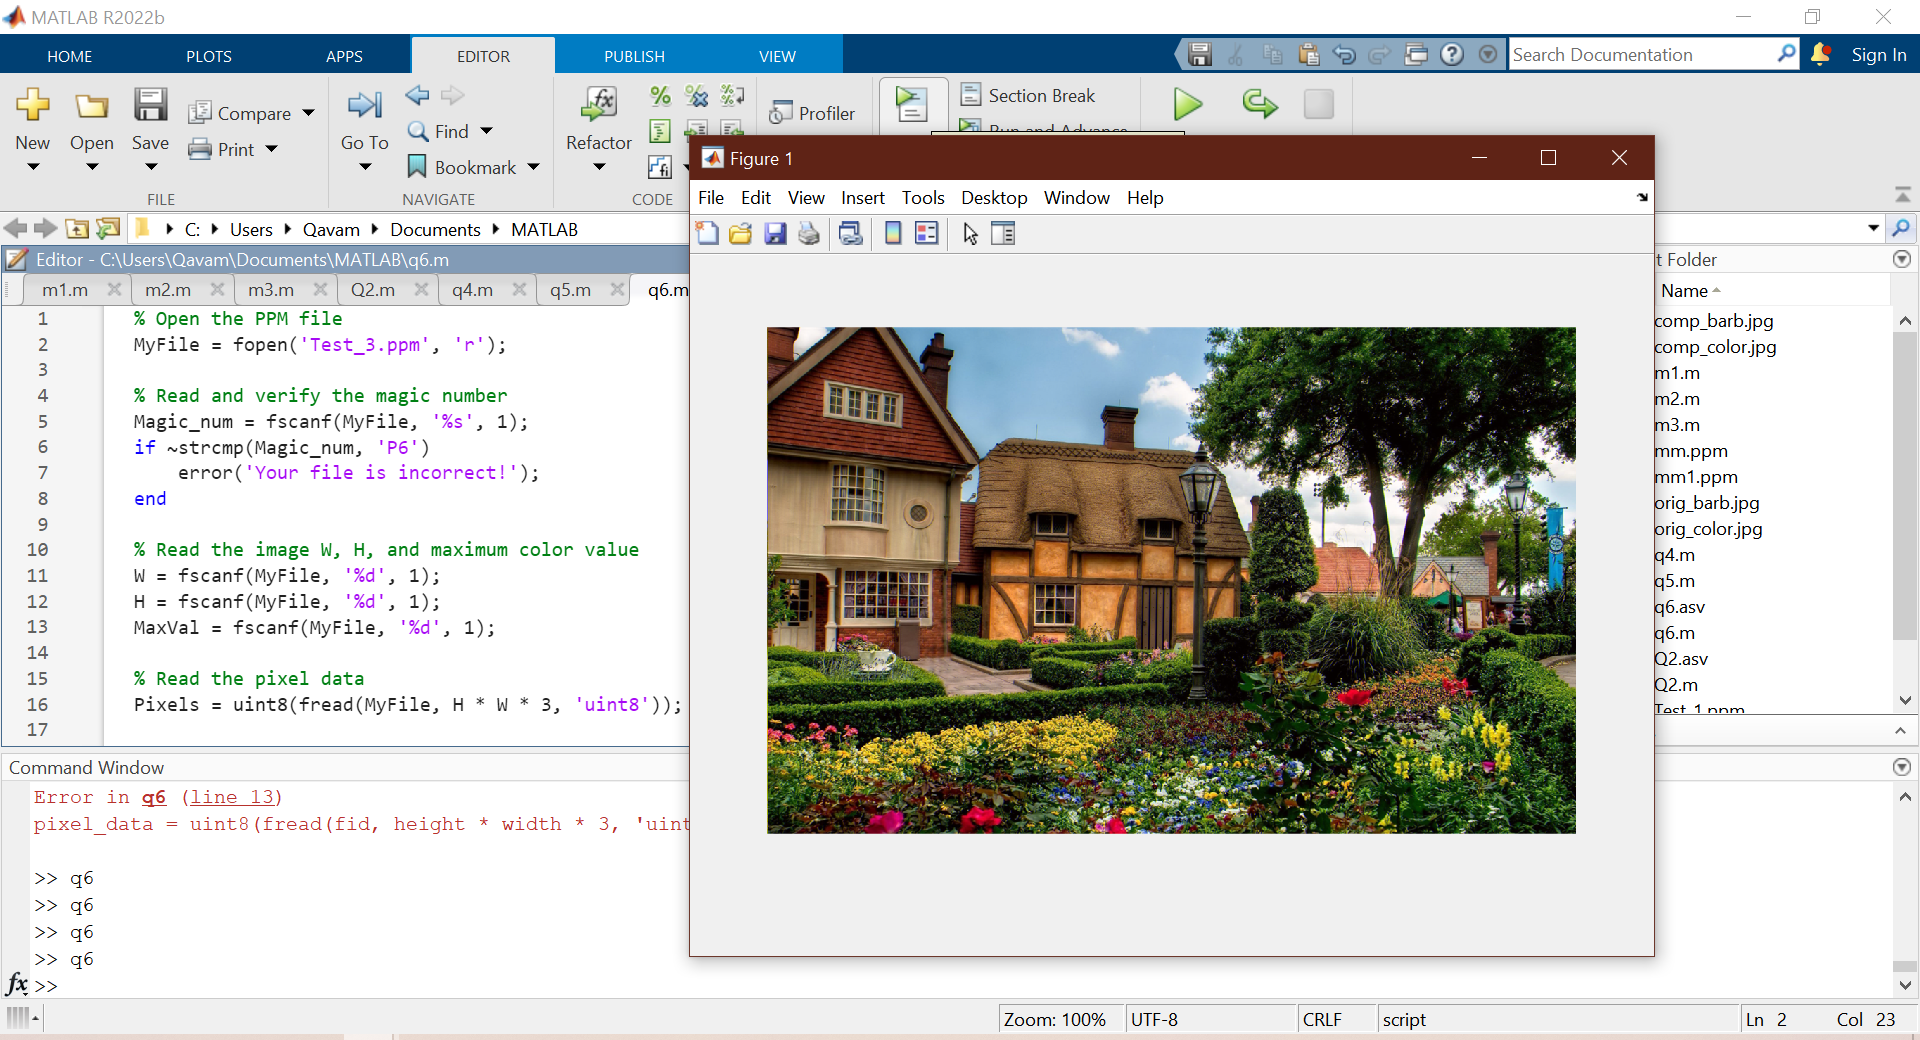
\includegraphics[width=0.9\textwidth]{3.png}
	\caption{1}
\end{figure}

	\section{تابع \lr{MSE}}
	
	\lr{\lstinputlisting[language=Matlab, showstringspaces=false, basicstyle=\ttfamily, backgroundcolor=\color{gray!20!white}, breaklines=true]{My_MSE.m}}

برای اطمینان از دقیق بودن محاسبات، تصاویر با استفاده از «\lr{im2double}» با دقت  اضافه در نظر گرفته می شوند. این تابع تصویر را با دقت دو برابر درنظر می گیرد و تضمین می‌کند که مقادیر پیکسل‌ها، به‌عنوان مقادیر ممیز شناور با دقت دوگانه، از 0 تا 1 نمایش داده می‌شوند. معمولا برای مسائل گوناگون پردازش تصویر که نیاز به کار با داده‌های نرمال‌شده دارند، این تابع مورد استفاده قرار می گیرد. سپس خطای مربع بین تصاویر اصلی و بازسازی شده با کم کردن مقادیر پیکسل تصویر بازسازی شده از تصویر اصلی و توان دو کردن نتیجه محاسبه می شود. و بعد میانگین مربعات خطا با میانگین مقادیر مربعات خطا در تمام پیکسل های تصویر محاسبه می شود. 

در نهایت، بسته به نوع تصویر، تعداد پیکسل ها مشخص می شود. اگر تصویر بیش از یک کانال داشته باشد، یک تصویر رنگی در نظر گرفته می شود و تعداد کل پیکسل ها از حاصل ضرب تعداد سطرها، ستون ها و کانال ها محاسبه می شود. اگر تصویر فقط یک کانال داشته باشد، آن را در مقیاس خاکستری یا سیاه و سفید در نظر می گیرند و تعداد کل پیکسل ها به سادگی تعداد عناصر موجود در تصویر است.
در نهایت، \lr{MSE} با ضرب میانگین مجذور خطا در تعداد کل پیکسل ها محاسبه می شود. \cite{5}
	
	\section{تابع \lr{PSNR}}
	
	\lr{\lstinputlisting[language=Matlab, showstringspaces=false, basicstyle=\ttfamily, backgroundcolor=\color{gray!20!white}, breaklines=true]{My_PSNR.m}}
	
	طبق سوال قبلی، پس از محاسبه \lr{MSE} < و تعیین بیشترین مقدار آن، با فرمول \lr{PSNR} مقدار این مؤلفه به دست می آید. مقدار \lr{PSNR} نشان دهنده کیفیت تصویر بازسازی شده در مقایسه با تصویر اصلی است و مقادیر بالاتر نشان دهنده کیفیت بهتر است. \cite{6}
	
	\begin{figure}[H]
		\centering
		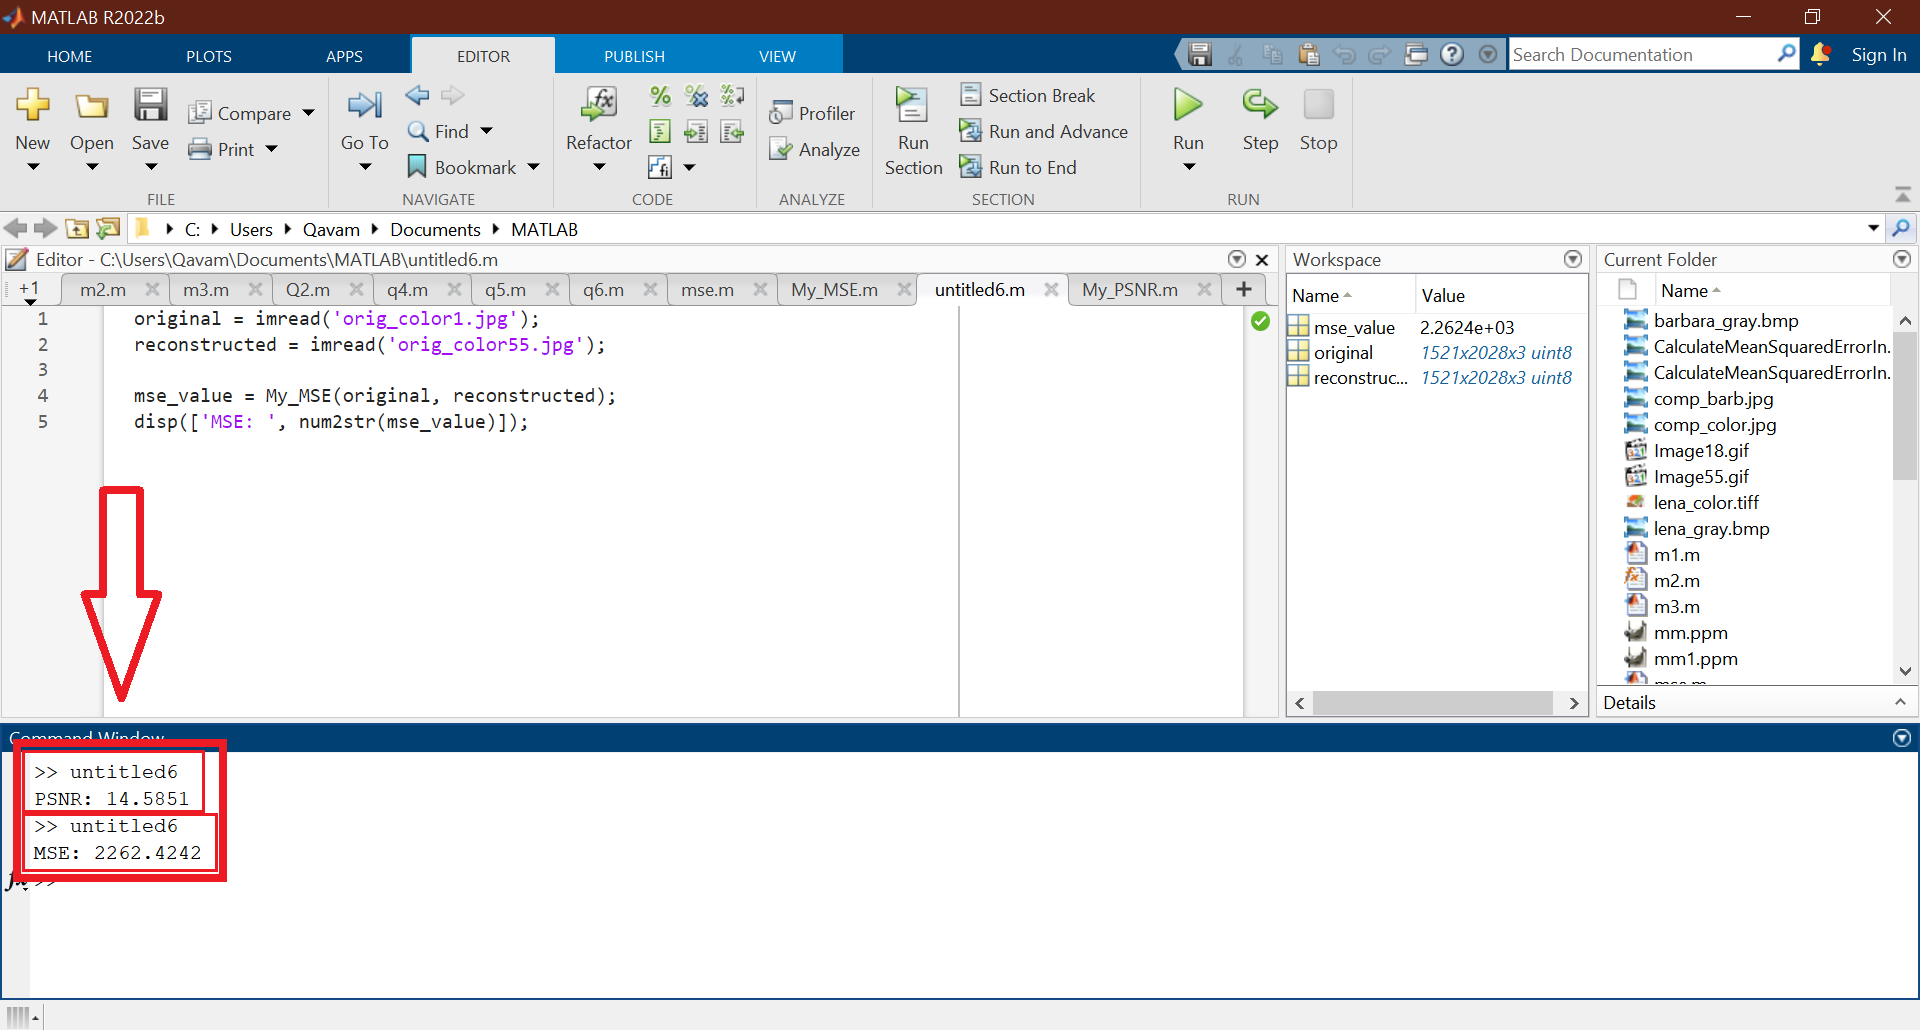
\includegraphics[width=0.9\textwidth]{4_5.png}
		\caption{نتایج سوال 4 و 5}
	\end{figure}
	
	
	
	\section{سوال \lr{Entropy}}
	
		\lr{\lstinputlisting[language=Matlab, showstringspaces=false, basicstyle=\ttfamily, backgroundcolor=\color{gray!20!white}, breaklines=true]{My_Entropy.m}}
	
پس از مشخص کردن داده ها، تابع '\lr{histcounts}' برای محاسبه توزیع احتمال داده های ورودی اجرا می شود و یک هیستوگرام از داده ها را محاسبه می کند و تعداد مقادیری که در هر \lr{bin} قرار می گیرند را برمی گرداند. با مشخص کردن آرگومان "\lr{Normalization}"، "\lr{Probability}"، شمارش برای به دست آوردن احتمال هر bin نرمال انجام می شود. سپس توزیع احتمال محاسبه شده در متغیر '\lr{prob}' ذخیره می شود که نشان دهنده احتمال وقوع هر مقدار، در داده های ورودی است. صفرها در بردار 'prob' که به محاسبه آنتروپی کمک نمی کنند، حذف می شوند. و در نهایت، محاسبه آنتروپی با استفاده از فرمول آن انجام می شود.\cite{7}
	

	 
	 
	 \section{\lr{rgb2gray}}
	 
	 
	 
	 \begin{figure}[H]
	 	\centering
	 	
	 	\subfigure[]{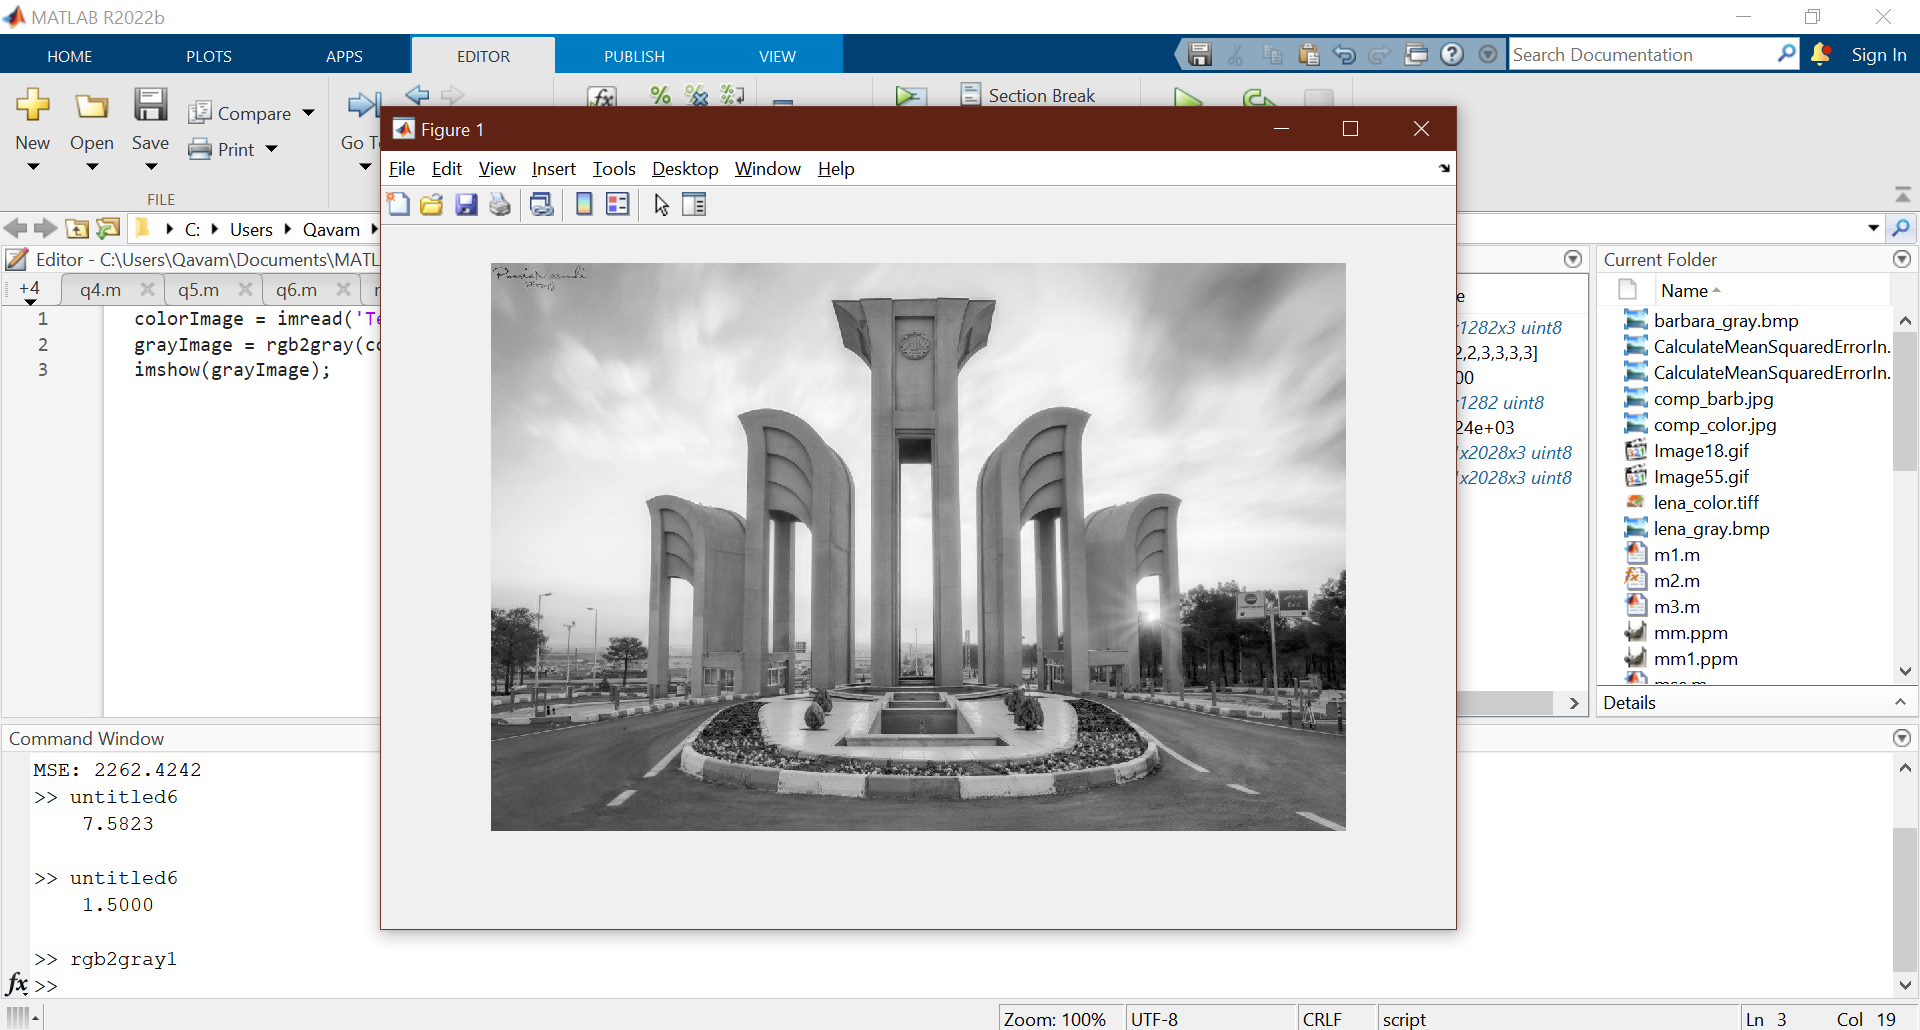
\includegraphics[width=0.3\textwidth]{g2.png}}
	 	\hfill
	 		\subfigure[]{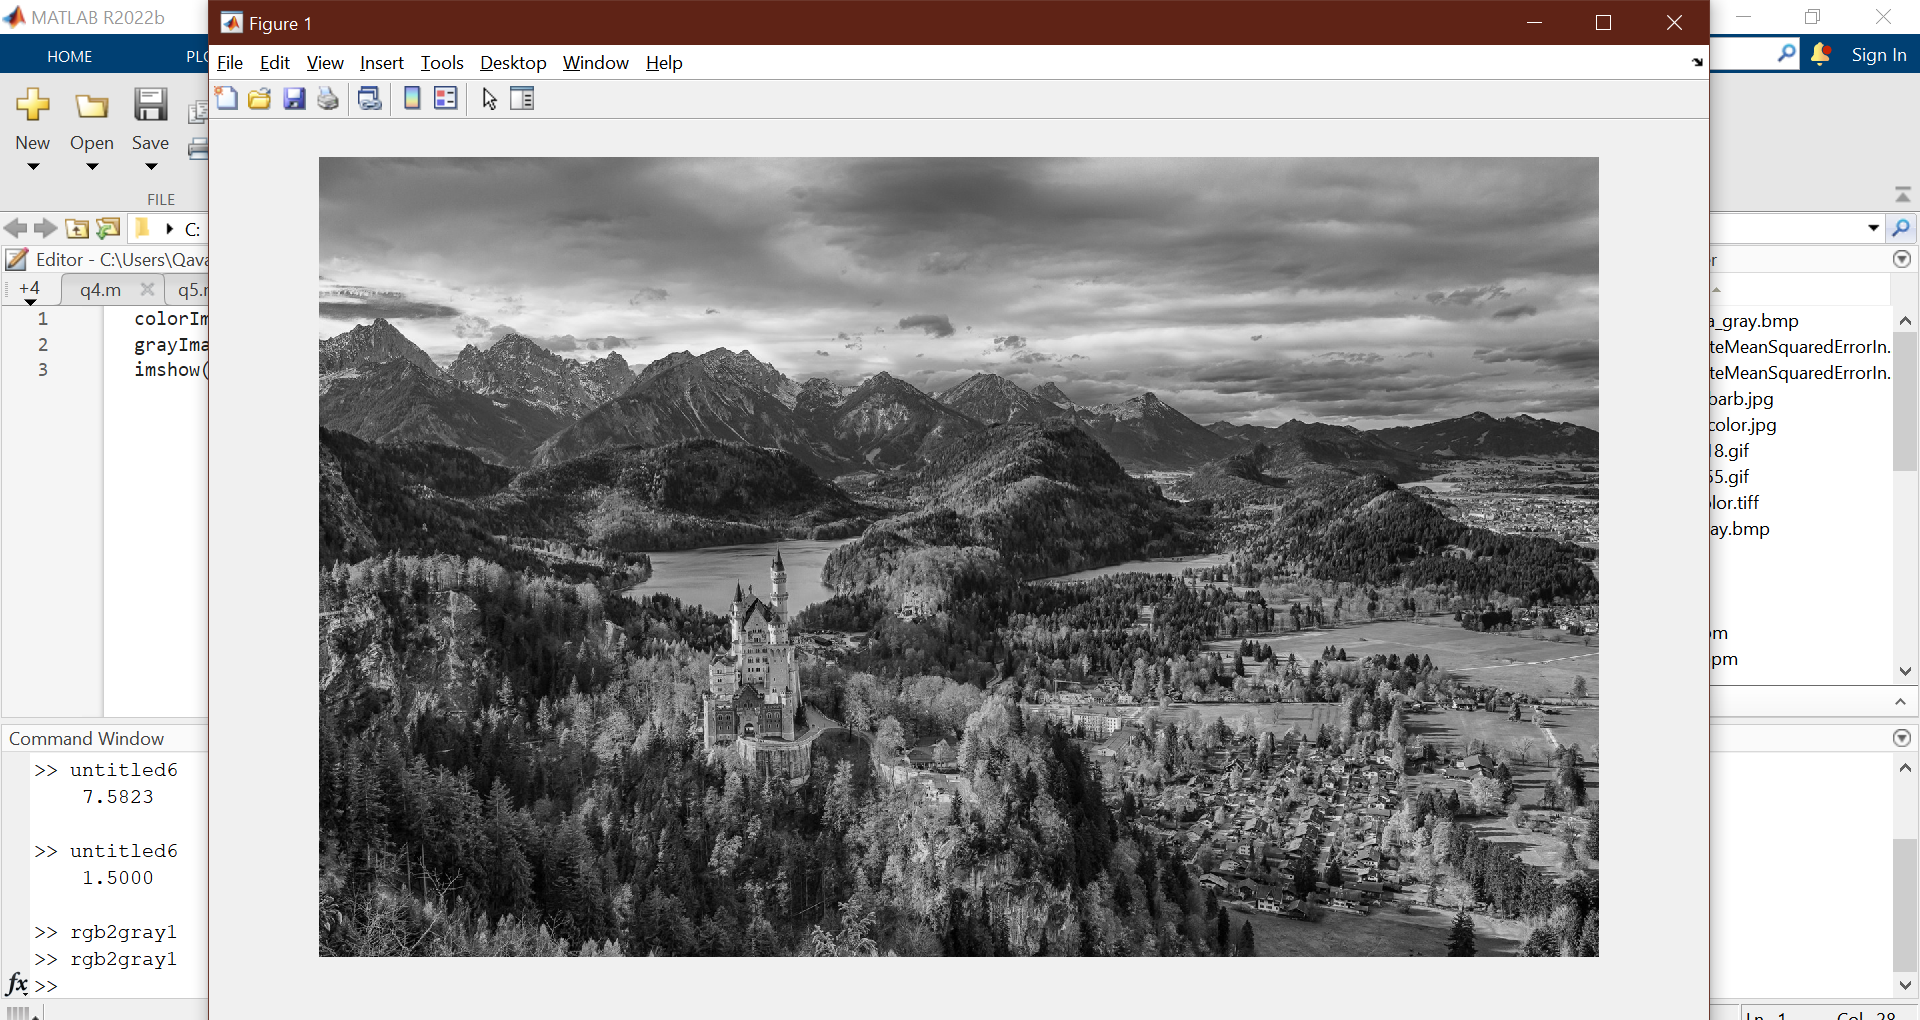
\includegraphics[width=0.3\textwidth]{g3.png}}
	 	\hfill
	 \subfigure[]{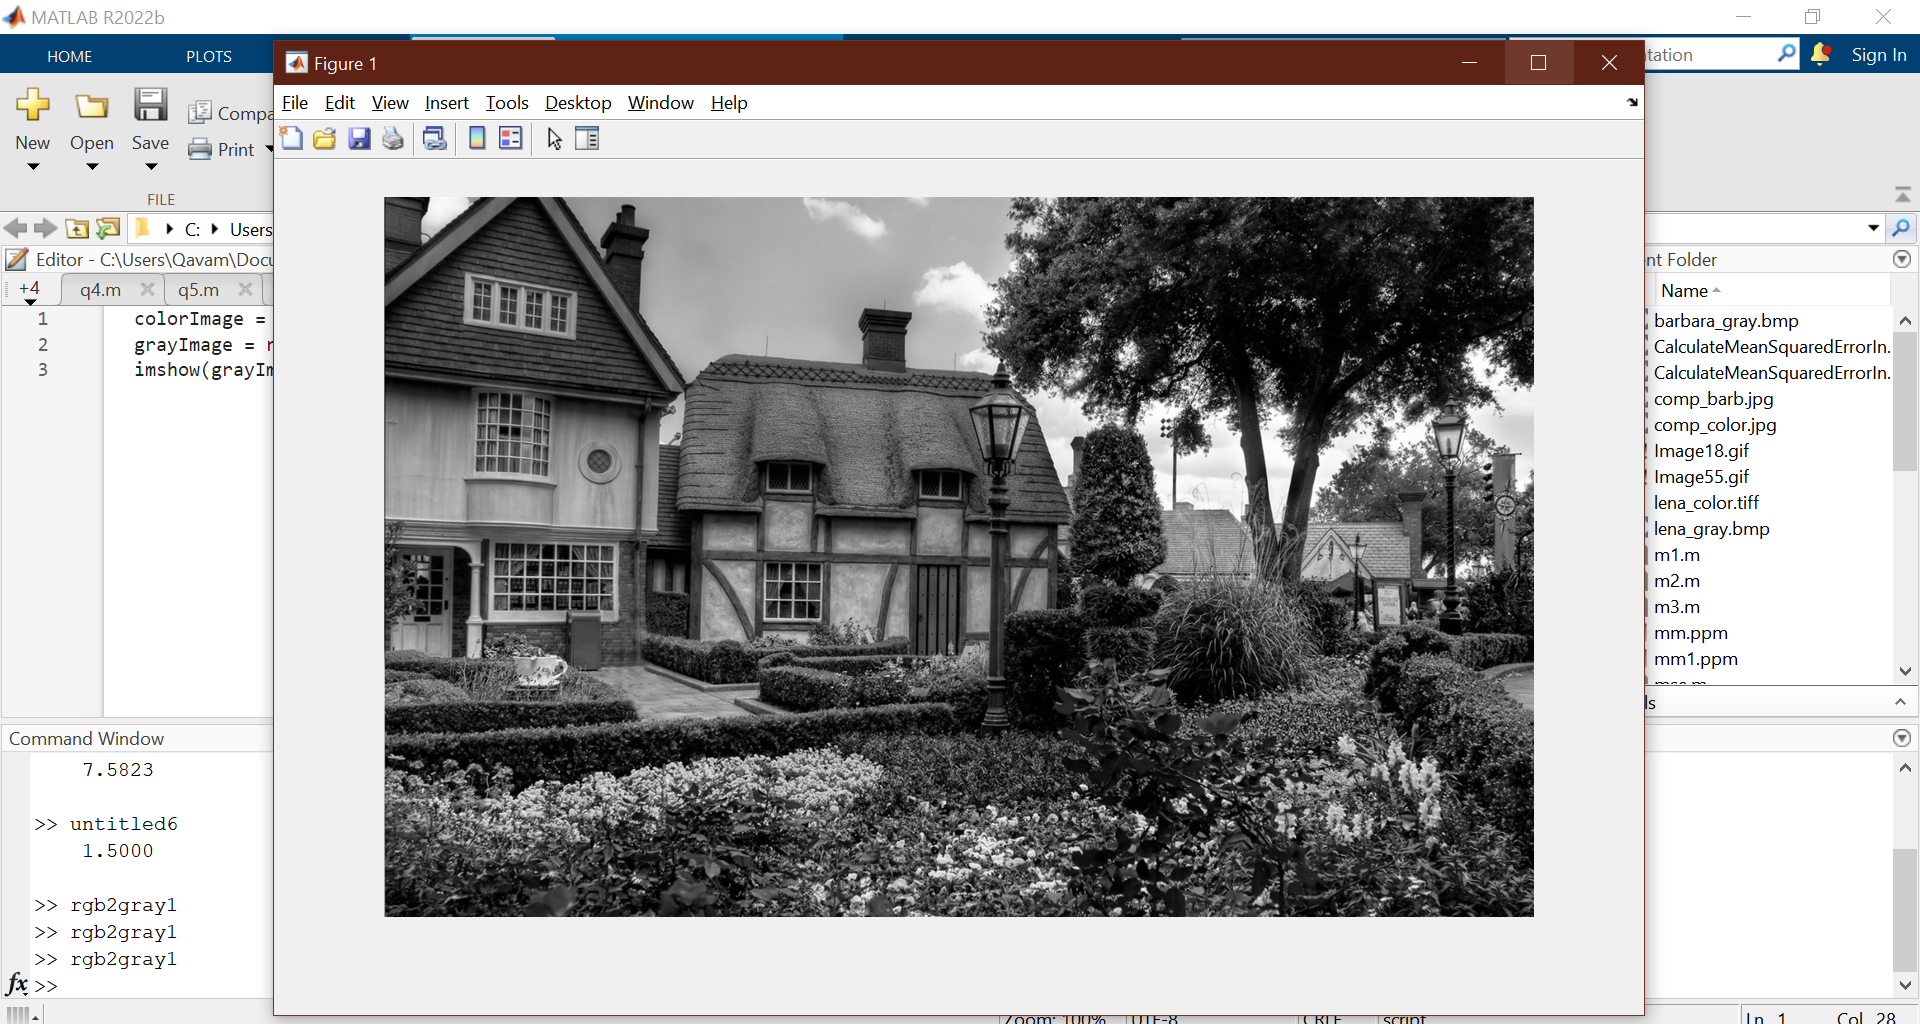
\includegraphics[width=0.3\textwidth]{g1.png}}
	 	
		\caption{نتایج}

	 \end{figure}
	 
	 کد جهت ذخیره فایل های جدید:
	\begin{latin}
	\begin{verbatim}
		colorImage = imread('Test_1.ppm');
		grayImage = rgb2gray(colorImage);
		imshow(grayImage);
		imwrite(grayImage,'Test_1G.ppm');
	\end{verbatim}
		\end{latin}
	
	
	\section{سوال هفتم}
	برای تبدیل یک تصویر رنگی به مقیاس خاکستری و در عین حال به حداکثر رساندن اطلاعات منتقل شده از کانال های رنگی، می توان از فرمول تبدیل روشنایی استفاده کرد. این فرمول مجموع وزنی کانال های رنگی را برای نمایش شدت تصویر در مقیاس خاکستری محاسبه می کند.\cite{8}
	
	مقادیر درخشندگی با استفاده از فرمول «$0.299 * R + 0.587 * G + 0.114 * B$» محاسبه می شود، که در آن R، G، و B به ترتیب کانال های قرمز، سبز و آبی تصویر رنگی هستند. ضرایب (وزن ها) برای تقریب درک انسان از روشنایی بر اساس سهم نسبی هر کانال رنگ انتخاب می شوند.\cite{8}
	
	با استفاده از این روش، اطلاعات هر سه کانال رنگی در تصویر خاکستری گنجانده می شود و تا حد امکان جزئیات و کیفیت بصری را از تصویر رنگی اصلی حفظ می کند.\cite{8}
	
	
	\lr{\lstinputlisting[language=Matlab, showstringspaces=false, basicstyle=\ttfamily, backgroundcolor=\color{gray!20!white}, breaklines=true]{convertToGrayscale.m}}
	
	
\begin{latin}
\begin{table}[H]
	\centering
	\arrayrulecolor{black}
	\begin{tabular}{|c|c|c|c|c|} 
		\cline{3-5}
		\multicolumn{1}{c}{}                                                                                &      & 1          & 2          & 3           \\ 
		\hline
		{\cellcolor[rgb]{0.6,0.941,0.624}}                                                                  & MSE  & 23218.7367 & 60321.8661 & 27030.9508  \\ 
		\hhline{|>{\arrayrulecolor[rgb]{0.6,0.941,0.624}}->{\arrayrulecolor{black}}----|}
		\multirow{-2}{*}{{\cellcolor[rgb]{0.6,0.941,0.624}}rgb2gray}                                        & PSNR & 4.4724     & 0.32606    & 3.8122      \\ 
		\hline
		{\cellcolor[rgb]{0.976,0.643,0.745}}                                                                & MSE  & 23222.9926 & 60341.3897 & 27034.7804  \\ 
		\hhline{|>{\arrayrulecolor[rgb]{0.976,0.643,0.745}}->{\arrayrulecolor{black}}----|}
		\multirow{-2}{*}{{\cellcolor[rgb]{0.976,0.643,0.745}}\textcolor[rgb]{0.078,0.09,0.094}{luminance~}} & PSNR & 4.4716     & 0.32465    & 3.8116      \\
		\hline
	\end{tabular}
\end{table}
\end{latin}
	
	\section{ سوال هشتم}
	کدنویسی و همیاری: \cite{9}
	\subsection{الف}

\begin{latin}
\begin{verbatim}

function CR = My_Unary_Encoder(Original_Filename_and_Path, Compressed_Filename_and_Path)
% Read the original file
original_data = imread(Original_Filename_and_Path);

% Convert the original data to a binary string using unary encoding
binary_string = '';
for i = 1:numel(original_data)
binary_string = strcat(binary_string, repmat('1', 1, original_data(i)));
binary_string = strcat(binary_string, '0');
end

% Write the binary string to a compressed file
fileID = fopen(Compressed_Filename_and_Path, 'w');
fwrite(fileID, binary_string, 'ubit1');
fclose(fileID);

% Calculate compression rate
original_file_info = dir(Original_Filename_and_Path);
compressed_file_info = dir(Compressed_Filename_and_Path);
original_file_size = original_file_info.bytes;
compressed_file_size = compressed_file_info.bytes;
CR = original_file_size / compressed_file_size;
end

***

function My_Unary_Decoder(Compressed_Filename_and_Path, Reconstructed_Filename_and_Path)
% Read the compressed file
fileID = fopen(Compressed_Filename_and_Path, 'r');
binary_string = fread(fileID, '*char');
fclose(fileID);

% Perform unary decoding to reconstruct the original data
reconstructed_data = [];
current_value = 0;
for i = 1:numel(binary_string)
if binary_string(i) == '1'
current_value = current_value + 1;
else
reconstructed_data = [reconstructed_data, current_value];
current_value = 0;
end
end

% Write the reconstructed data to the output file
imwrite(uint8(reconstructed_data), Reconstructed_Filename_and_Path);
end

\end{verbatim}
\end{latin}
	
	
	\subsection{ب}
	صفر است.
	
	\subsection{ج}
	
	\begin{latin}

% \usepackage{colortbl}
% \usepackage{hhline}


\begin{table}[H]
	\centering
	\begin{tabular}{|l|l|l|l} 
		\hhline{~--~}
		\multicolumn{1}{l|}{}                        & {\cellcolor[rgb]{0.957,0.745,0.745}}CR & {\cellcolor[rgb]{0.643,0.663,0.957}}MSE &   \\ 
		\hhline{|---~}
		{\cellcolor[rgb]{0.604,0.941,0.58}}Angio.bmp &                                        &                                         &   \\ 
		\hhline{|---~}
		{\cellcolor[rgb]{0.8,1,0.6}}Scenery.bmp      &                                        &                                         &   \\ 
		\hhline{|---~}
		{\cellcolor[rgb]{1,0.847,0.722}}Text.txt     &                                        &                                         &   \\
		\hhline{|---~}
	\end{tabular}
\end{table}

	\end{latin}
	
	\subsection{د}
	
\begin{latin}
	\begin{verbatim}
		
	function CR = My_Unary_Encoder(Original_Filename_and_Path, Compressed_Filename_and_Path)
	% Read the original image
	original_data = imread(Original_Filename_and_Path);
	
	% Perform histogram equalization
	equalized_data = histeq(original_data);
	
	% Convert the equalized data to a binary string using unary encoding
	binary_string = '';
	for i = 1:numel(equalized_data)
	binary_string = strcat(binary_string, repmat('1', 1, equalized_data(i)));
	binary_string = strcat(binary_string, '0');
	end
	
	% Write the binary string to a compressed file
	fileID = fopen(Compressed_Filename_and_Path, 'w');
	fwrite(fileID, binary_string, 'ubit1');
	fclose(fileID);
	
	% Calculate compression rate
	original_file_info = dir(Original_Filename_and_Path);
	compressed_file_info = dir(Compressed_Filename_and_Path);
	original_file_size = original_file_info.bytes;
	compressed_file_size = compressed_file_info.bytes;
	CR = original_file_size / compressed_file_size;
	end

\end{verbatim}
\end{latin}
	
	\subsection{ه}
	
	\begin{latin}
		\begin{table}[H]
			\centering
\begin{tblr}{
		cell{1}{1} = {c=2}{c},
		cell{1}{3} = {ScreaminGreen},
		cell{1}{4} = {Canary},
		cell{1}{5} = {CottonCandy},
		cell{2}{1} = {c=2}{c},
		cell{3}{1} = {c=2}{c},
		cell{4}{1} = {r=8}{BilobaFlower,c},
		cell{12}{1} = {r=8}{Cherub},
		vlines,
		hline{1-4,12,20} = {-}{},
		hline{5-11,13-19} = {2-5}{},
	}
	File Name                                     &                            & Text.txt & Scenery.bmp & Angio.bmp \\
	Entropy                                       &                            &          &             &           \\
	Coding Redundancy                             &                            &          &             &           \\
	\begin{sideways}Unary Code\end{sideways}      & Compressed Data Size (BPS) &          &             &           \\
	& Dictionary Size (BPS)      &          &             &           \\
	& Total Size (BPS)           &          &             &           \\
	& Compression Ratio          &          &             &           \\
	& Encoding Time              &          &             &           \\
	& Decoding Time              &          &             &           \\
	& MSE                        &          &             &           \\
	& PSNR                       &          &             &           \\
	\begin{sideways}Proposed Method\end{sideways} & Compressed Data Size (BPS) &          &             &           \\
	& Dictionary Size (BPS)      &          &             &           \\
	& Total Size (BPS)           &          &             &           \\
	& Compression Ratio          &          &             &           \\
	& Encoding Time              &          &             &           \\
	& Decoding Time              &          &             &           \\
	& MSE                        &          &     56        &           \\
	& PSNR                       &          &             &           
\end{tblr}
\end{table}
	
	\end{latin}
	

	
	\newpage
	
	\section*{منابع}
	\renewcommand{\section}[2]{}%
	\begin{thebibliography}{99} 
		
		\begin{latin}
		
		
		\begin{LTRitems}
			
			\resetlatinfont
			

			
				\bibitem{1} 
				\url{https://en.wikipedia.org/wiki/Netpbm}
				
					\bibitem{2} 
					\url{https://paulbourke.net/dataformats/ppm/}
					
						\bibitem{3} 
						\url{https://prasannk.tripod.com/imgformats.htm}
						
						\bibitem{5} 
						\url{https://github.com/jiny2001/dcscn-super-resolution/issues/9}
						
						\bibitem{4} 
						\url{https://www.mathworks.com/matlabcentral/answers/1596014-how-i-can-read-image-with-ppm-format-without-imread-and-design-ppm-reader}
						
						\bibitem{6}
						\url{https://www.mathworks.com/matlabcentral/answers/504512-psnr-calculation-without-using-function}
						
						\bibitem{7}
						\url{https://www.mathworks.com/matlabcentral/answers/42142-entropy-of-a-signal}
						
						
						\bibitem{8}
						\url{http://docs-hoffmann.de/gray10012001.pdf}
						
						\bibitem{20}
						\rl{با سپاس از \lr{ChatGPT :)}}
						
						
		\end{LTRitems}
	\end{latin}
		
	\end{thebibliography}
	
	
\end{document}